\section{Evaluation}
\label{sec.exp}

Our experimental study focuses on the following questions:

1. \textbf{Effectiveness and efficiency of \system}: How does \system compare with other Transformer-based methods and traditional timeseries representation learning methods in accuracy and efficiency?

% 2. \textbf{Efficiency of \system}:
% How does \system compare with other Transformer-based methods in term of efficiency?

%3. \textbf{Effectiveness of Pretraining}: How does the self-supervised pretraining task benefit the downstream tasks?

2. \textbf{Ablation Study}: How do the key techniques of \system work?

\subsection{Experimental Setup}
\label{sec.exp.setup}
\noindent\textbf{Datasets.}
We evaluate \system on classification and imputation tasks using 5 multi-variate and 3 uni-variate timeseries datasets.

\begin{compactitem}
\item
\textit{\textbf{WISDM}}~\cite{weiss2019smartphone} is a popular multivariate timeseries dataset generated from the accelerometer in the mobile phone.
The subjects performed 18 daily activities (e.g. walking, jogging). The dataset was collected from 51 subjects and the sampling rate is 20 Hz.


\item
\textit{\textbf{HHAR}} dataset~\cite{stisen2015smart} contains sensing data of accelerometer collected
from 9 users performing 5 activities with 12 different smartphones (varying in sampling rate). This increases the complexity of the task and thus can test the model’s robustness.

%, namely climbing up, climbing down, jumping, lying, running, sitting, standing, and walking
\item
{\textit{\textbf{RWHAR} RealWorld HAR}} dataset~\cite{sztyler2016body} covers 15 subjects performing 8 locomotion-style activities. Each subject wears the sensors for approximately ten minutes. The sampling rate is 50 Hz.

\item
\textit{\textbf{ECG}} dataset~\cite{liu2018open} consists
of 10,000 EEG recordings for arrhythmia classification. Each recording has an uncertain length ranging from 6 to 60 seconds sampled at 500 Hz. The ECG recordings correspond to 9 types of heart problems such as atrial fibrillation (AF) and premature atrial contraction (PAC), etc. 

\item
{\textit{\textbf{MGH}}}~\cite{DBLP:journals/pvldb/CaoTAJYLGSBSCWM19} is a EEG dataset collected by Mass. General Hospital. Each timeseries corresponds to the EEG data observed from one patient during their stay in ICU for a couple of days. The EEG monitoring produced data with 20 channels. The sampling rate is 200 HZ. So it produces very long timeseries.

\item
{\textit{\textbf{WISDM*/HHAR*/RWHAR*}}}
are three uni-variate datasets derived by picking one channel from \textit{WISDM/HHAR/RWHAR}.

\end{compactitem}


\noindent\textbf{Training/Validation Data Generation.}
We apply a sliding window on the raw timeseries to get training/validation samples. 
%The overlap rate is set as 0.5 for supervised training data and 0.8 for unsupervised training data.
The size of the sliding window is set as 200 on small datasets (WISDM, HHAR, RWHAR), 2000 on medium size dataset (ECG), and 10,000 on the large dataset (MGH). Table~\ref{tab.dataset} shows the statics of the generated datasets. They are randomly split into training/validation set in a proportion of 0.9/0.1. 
In ``pretraining + few-label finetuning'' scenario, we use 100 labeled data per class for finetuning. We guarantee that training set does not overlap with the validation set.

\begin{table}[htbp]
\vspace{-3mm}
\centering
\footnotesize
\begin{tabular}{c|c|c|c|c|c}
\toprule
    Dataset & Train. Size & Valid. Size & Length & Channel & Classes \\
    \hline
    WISDM & 28,280 & 3,112 & 200 & 3 & 18\\
    HHAR & 20,484 & 2,296 & 200 & 3 & 5\\
    RWHAR & 27,253 & 3,059 & 200 & 3 & 8\\
    ECG & 31,091 & 3,551 & 2000 & 12 & 9\\
    MGH & 8,550 & 950 & 10000 & 21 & N/A\\
 \bottomrule
\end{tabular}
\caption{The statistics of the datasets}
\label{tab.dataset}
\vspace{-7mm}
\end{table}

%TST showed that Transformer based method has advantages over other deep-learning based methods or traditional methods on the task of timeseries regression and classification. TST explored self-supervised pretraining with unlabeled timeseries.

\noindent\textbf{Alternative Methods.} 
We compare \system against the SOTA Transformer based timeseries representation learning method {\bf TST}~\cite{DBLP:conf/kdd/ZerveasJPBE21}. 
To evaluate our group attention (referred to as \textbf{Group Attn.}), we develop three baselines by replacing the group attention component in \system with the classic vanilla Self-Attention~\cite{DBLP:conf/nips/VaswaniSPUJGKP17}(referred to as \textbf{Vanilla}) and two SOTA methods that reduce the complexity of self-attention by approximation in NLP, namely, Performer~\cite{choromanski2020rethinking} (referred to as \textbf{Performer}) and Linformer~\cite{wang2020linformer} (referred to as \textbf{Linformer}). 
Similar to our proposed Group Attn., Vanilla, Performer, Linformer all use \system's time-aware convolution operation (Sec.~\ref{sec.rita}) to turn timeseries segments into input feature vectors.

We also compare Group Attn. against \textbf{GRAIL}~\cite{paparrizos2019grail}, which is the SOTA of the non-deep learning methods for timeseries representation learning. GRAIL supports classification tasks by feeding the learned representations into a Support-Vector Machine~\cite{cortes1995support} or K-Nearest Neighbor~\cite{fix1989discriminatory} classifier. 
Note GRAIL only targets {\bf uni-variate} timeseries and cannot support imputation tasks.

%\srm{Does RITA do anything in the Vanilla case?  or is this just a off the self self attention mechansim?  I'm unclear what part of RITA is left after we "plug in" vanilla / linformer / performer.}

%, such as Rocket\cite{DBLP:journals/datamine/DempsterPW20}, ResNet\cite{he2016deep}, InceptionTime\cite{ismail2020inceptiontime}
% \begin{compactitem}

% \item
% {\textit{\textbf{TST} Time Series Transformer}}~\cite{DBLP:conf/kdd/ZerveasJPBE21} is the SOTA Transformer-based time series analytics method. It shows Transformer-based method has advantages over other deep-learning based methods or traditional method on the task of timeseries regression and classification. It also explored self-supervised pretraining with unlabeled time series.

% \item
% \textit{\textbf{Vanilla}}. Vanilla Self-Attention~\cite{DBLP:conf/nips/VaswaniSPUJGKP17} computes the pairwise attention scores with a time/space cost quadratic to the length of the timeseries. 
% %Although \textit{\textbf{Vanilla}} produces precise attention scores, its scalability is limited by the heavy cost.

% \item
% \textit{\textbf{Linformer}}. Linformer~\cite{wang2020linformer} projects the query, key and value matrices which sometimes are low-ranked into smaller matrices before attention computation.
% The deficiencies of \textit{\textbf{Linformer}} are: (1) The size of the projected matrix needs careful tuning by the users; (2) The projection operation introduces extra model parameters.

% \item
% \textit{\textbf{Performer}}. Performer~\cite{choromanski2020rethinking} uses linear functions to approximate the non-linear Softmax function, making attention computation commutative and thus faster.% When the sequence length is far greater than the dimension of the embedding vectors, Performer benefits from changing the order of matrix multiplication.

% \end{compactitem}

\noindent\textbf{Methodology.}
We mainly focus on two downstream tasks:

(1) \textbf{Classification}. 
First, we train Group Attn. and the baselines with full labels from scratch to test the effectiveness of \system framework and the approximation quality of our group attention. 

%On uni-variate datasets, GRAIL is chosen as the baseline. On multi-variate datasets, TST/Vanilla/Performer/Linformer are chosen as the baselines, because GRAIL only targets uni-variate timeseries.

Second, to measure the effectiveness of self-supervised pretraining, we evaluate the accuracy of training on few labeled timeseries with/without pretraining on large scales of unlabeled timeseries. 
To be specific, we split the training set into a {\it pretraining} set and a {\it finetuning} set, with very few data in the latter (100 labeled samples per class in our experiment). 
We train the model on the cloze pretraining task with a mask rate $p=0.2$. 
Then we train two classification models using the finetuning set, either based on the pretrained version or from scratch. We repeat the experiment 5 times with random data splits and report the median accuracy. 

%We conduct the experiment on multi-variate datasets with TST/Vanilla/Performer/Linformer as baselines because GRAIL doesn't support pretraining.\jm{revised}

(2) \textbf{Imputation}. We run the imputation task on the datasets used in classification as well as the large unlabeled MGH dataset, and measure the mean square error and absolute imputation error. To get timeseries with missing values, we randomly mask the values with an expected mask rate of $p=0.2$. The masked values are replaced with a special value. 

Finally, to evaluate Group Attn.'s benefit on {\bf efficiency}, the total time of forward computation, backward propagation, and grouping are measured for all methods in all the experiments. 

To save space, we only report the average training time per epoch here and refer readers to Appendix~\ref{sec.sup.evaltime} for the inference time.

We first compare against the Transformer-based methods on multi-variate datasets (sec.~\ref{sec.exp.effective}, \ref{sec.exp.efficiency}), then compare against the non-deep learning method GRAIL on uni-variate datasets (sec.~\ref{sec.exp.univariate}).

\noindent\textbf{Configuration.} Please refer to Appendix~\ref{appendix.exp} for the experiment configuration and hyper-parameter settings.

\begin{figure}[t]
%\vspace{2mm}
    \centering
    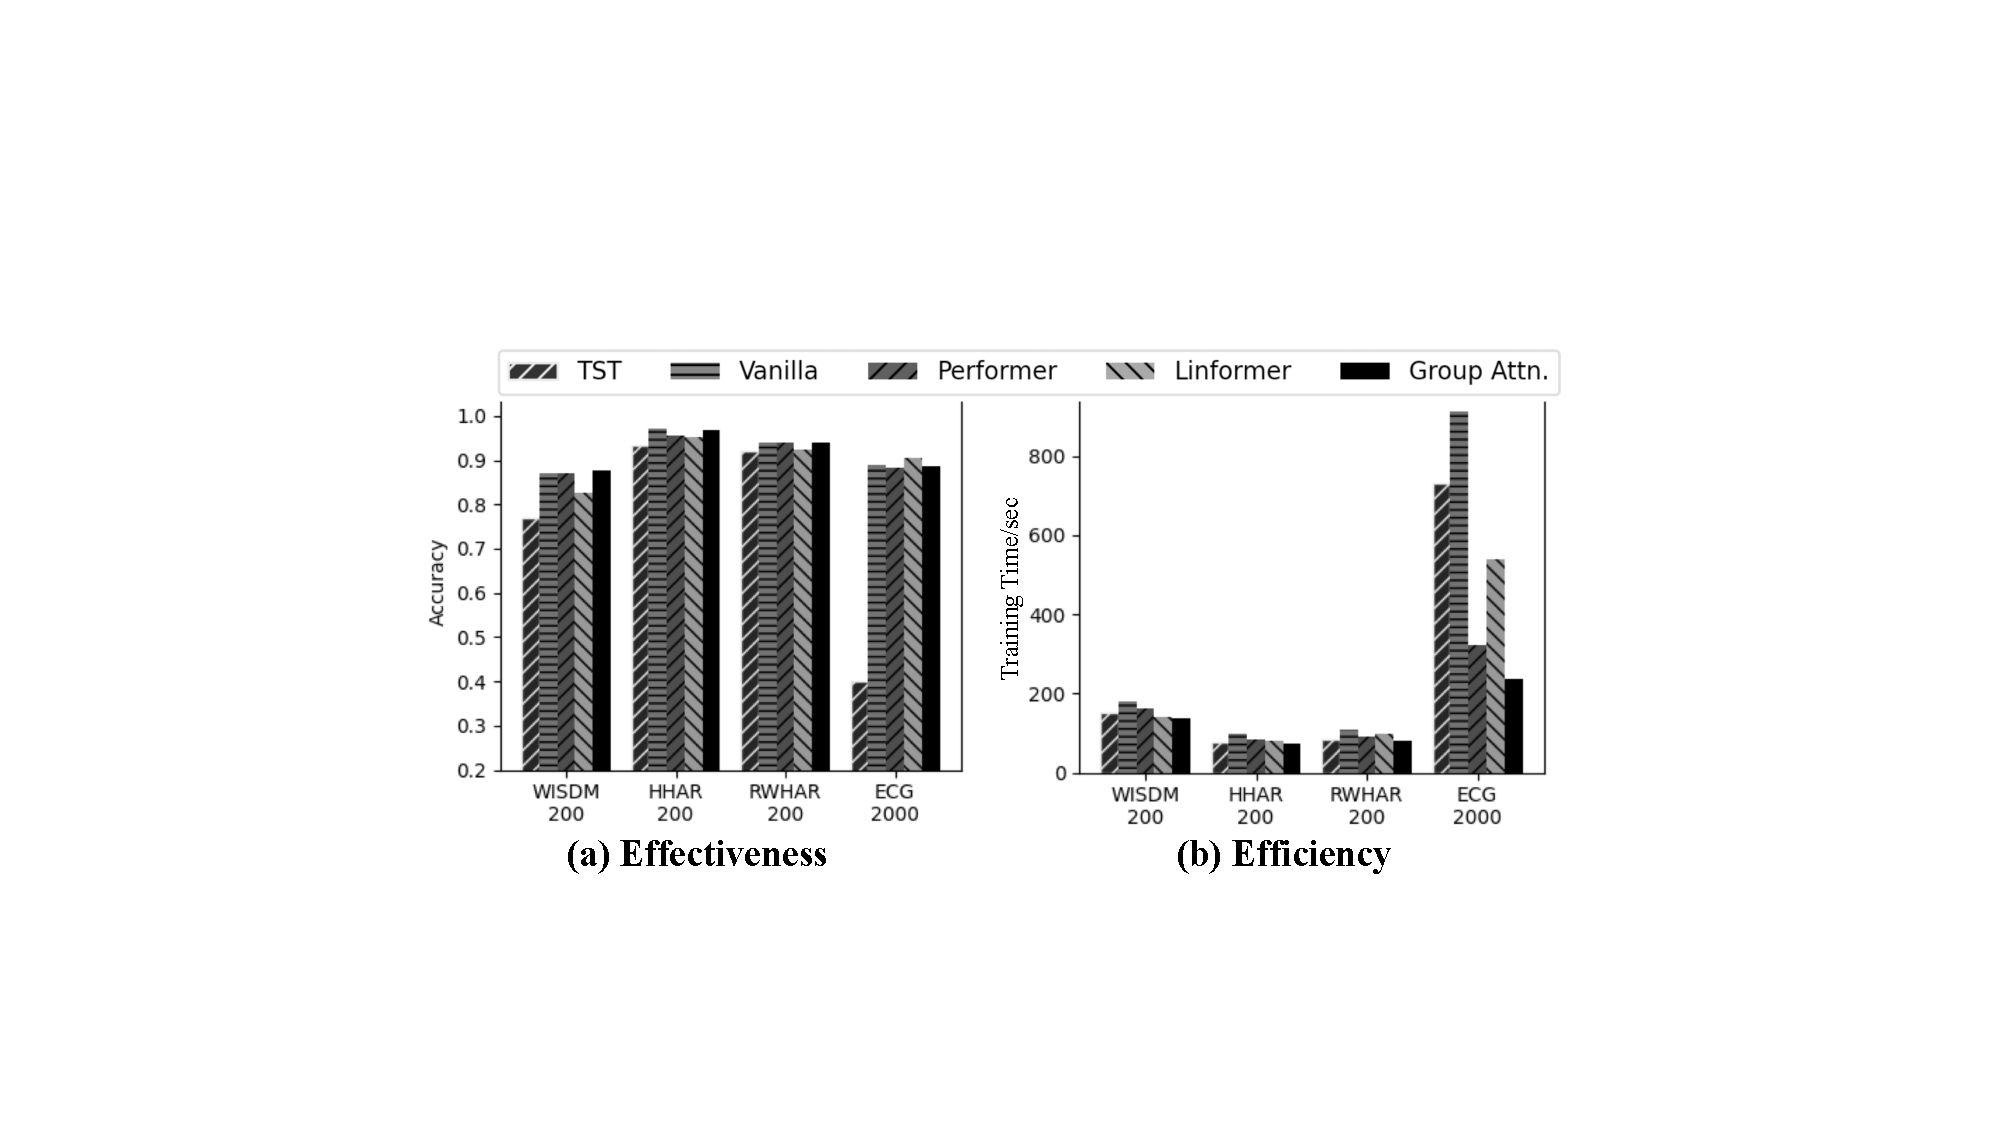
\includegraphics[width=1.0\columnwidth]{figures/cls.pdf}
    \vspace{-6mm}
    %\setcaptionwidth{3.5in}
    \caption{Full-label classification results (multi-variate data).}
    %Efficiency is measured by the average training time per epoch. \jm{revised}
    \label{fig.full}
    \vspace{-6mm}
\end{figure}

\begin{table*}[t]
\vspace{-2mm}
\centering
\footnotesize
\begin{tabular}{cc|cc|cc|cc|cc|cc}
\toprule
\multirow{2}{*}{Dataset} &  \multirow{2}{*}{Length} &
\multicolumn{2}{c}{TST~\cite{DBLP:conf/kdd/ZerveasJPBE21}}& \multicolumn{2}{c}{Vanilla} & \multicolumn{2}{c}{Performer} & \multicolumn{2}{c}{Linformer} & \multicolumn{2}{c}{Group Attn.}\\
 \cline{3-12}
 &   &  MSE & Time/s & MSE & Time/s  & MSE & Time/s  & MSE & Time/s  & MSE & Time/s \\
 \hline
 WISDM & 200 & 13.30 & 150.3 & \underline{\textbf{3.240}} & 178.1 & 3.449 & 162.6 & 3.852 & 141.9 & 3.277 & \underline{\textbf{136.7}}  \\
 HHAR & 200 & 1.085 & 78.2 &  \underline{\textbf{0.2968}} &  97.4 & 0.2980 & 82.6 & 0.3198 & 81.1 & 0.2974 & \underline{\textbf{73.3}} \\
 RWHAR & 200 & 0.0882 & 83.9 & \underline{\textbf{0.0478}} & 108.1 & 0.0489 & 89.1 & 0.0572 & 98.4 & \underline{\textbf{0.0478}} & \underline{\textbf{81.3}}\\
  ECG & 2000 & 0.0905 &	696.3 &	0.0037	& 857.9 & 	\underline{\textbf{0.0033}} &	270.2 &	0.0035 &	291.38 &	0.0038 &	\underline{\textbf{164.36}}\\
 MGH  & 10000 & N/A & N/A & N/A & N/A & \underline{\textbf{0.00014}} & 356.2 & 0.00088 & 404.9 & 0.00042 & \underline{\textbf{54.4}} \\
 \bottomrule
\end{tabular}
%\setcaptionwidth{5in}
\caption{Imputation results (multi-variate data). The best results are marked with \underline{bold}.}
\label{tab.imputationMulti}
\vspace{-5mm}
\end{table*}



















\begin{table*}[t]
\vspace{-2mm}
\centering
\footnotesize
\begin{tabular}{cc|cc|cc|cc|cc|cc}
\toprule
\multirow{2}{*}{Dataset} &  \multirow{2}{*}{Pretrain Size} &
\multicolumn{2}{c}{TST~\cite{DBLP:conf/kdd/ZerveasJPBE21}}& \multicolumn{2}{c}{Vanilla} & \multicolumn{2}{c}{Performer} & \multicolumn{2}{c}{Linformer} & \multicolumn{2}{c}{Group Attn.}\\
 \cline{3-12}
 &   &  Scratch & Pre. & Scratch & Pre. & Scratch & Pre. & Scratch & Pre. & Scratch & Pre.\\
 \hline
 WISDM & 62,231 & 49.13\% & 50.03\% & 66.16\% & \underline{\textbf{75.89\%}} & 66.09\% & 73.97\% & 50.12\% & 67.44\% & 62.56\% & 75.06\%  \\
 HHAR & 68,294 & 72.56\% & 75.30\% & 75.60\% & 81.35\% & 76.52\% & 80.70\% & 65.94\% & 76.52\% & 76.17\% & \underline{\textbf{82.62\%}}\\
 RWHAR & 63,599 & 69.46\% & 80.41\% & 85.68\% & 91.14\% & 87.54\% & \underline{\textbf{91.33\%}} & 81.03\% & 86.33\% & 86.13\% & 89.63\%\\
 ECG  & 561,358 & 20.98\% & 27.99\% & 42.05\% & 46.16\% & 43.34\% & 45.58\% & 27.19\% & 31.34\% & 42.58\% & \underline{\textbf{46.39\%}} \\
 \bottomrule
\end{tabular}
%\setcaptionwidth{5in}
\caption{Pretrain + few-label finetuning results. The best results are marked with \underline{bold}.}
\label{tab.pretrain}
\vspace{-5mm}
\end{table*}

\subsection{Effectiveness: Transformer-Based Methods}
\label{sec.exp.effective}
We first evaluate the quality of the models trained with full labels from scratch. We then show how the pretraining of \system increases the accuracy of the downstream tasks. 

\subsubsection{full-label training (Multi-variate classification) \nopunct}\ \\
Results shown in Figure~\ref{fig.full}(a) get us the following observations: 

\textbf{(1) \system's advantage over TST.} On all four datasets for the classification tasks,  Group Attn. and the other three baselines that use \system architecture (Vanilla, Performer, and Linformer) outperform TST. In particular, Group Attn. outperforms TST by 49 percentage points on the ECG dataset (88.48\% vs 39.93\%) with long timeseries.
Two deficiencies in TST may cause its poor performance on the long timeseries. Firstly, TST concatenates the output embedding vector of each time stamp, then uses a linear classifier to do classification on the concatenated vector. When the timeseries is long, the linear classifier has so many parameters that it tends to overfit easily. Secondly, TST replaces Layer Normalization in vanilla Transformer with Batch Normalization. 
When the timeseries is long, it can only accommodate a small number of timeseries in each batch, leading to bias in Batch Normalization.
%As a result, methods using the \system architecture outperform TST on all four classification 
% datasets, especially on ECG. 

\textbf{(2) Group-attention's advantage over other attention mechanisms.} 
Group Attn. is better than Performer and Linformer on 3 out of 4 datasets for classification. Although Linformer works slightly better than Group Attn. on the ECG dataset (90.37\% vs 88.84\%), its performance is the worst in all other cases compared to any other \system-based methods.
Vanilla computes the attention scores precisely. Thus it is expected to work well. However, Group Attn. outperforms Vanilla on WISDM (87.50\% vs 86.95\%) and is very close to it on other 3 datasets.
This suggests that group attention's approximation quality is good.

%and sometimes even improve the performance, because a proper grouping can provide the model a hint that some windows are of similar semantics/under similar contexts.

\subsubsection{pretraining + few label finetune (Multi-variate classification)\nopunct}\ \\
The results shown in Table~\ref{tab.pretrain} get us the following observation: 

\textbf{(1) Pretraining is effective.} Pretraining always leads to better accuracy than training with a few labels from scratch. In particular, on WISDM data all the methods using \system architecture increase the accuracy by at least 10\%. This is impressive considering we do not have a very large unlabeled pre-training set to use.

\textbf{(2) \system's advantage over TST.} our Group Attn. and other three baselines using \system architecture (Vanilla, Performer, and Linformer) significantly outperform TST on all four classification datasets by 25 percentage points.

\textbf{(3) Group Attention's advantage over other attention mechanisms.} Group Attn. is better than Performer and Linformer on 3 out of 4 datasets. When compared to Vanilla, Group Attn. is better on HHAR and ECG, and comparable on the other two, further confirming its high quality on approximation. 
Further, we notice that Linformer struggles in this setting: in average its accuracy is worse than Vanilla by 8.22\% and Group Attn. by 8.01\%. 
This is because the low-rank projection operation introduces extra model parameters, making Linformer more easily overfit, while overfitting is especially harmful when there are only a few labeled training samples.

\subsubsection{full-dataset training (Multi-variate imputation)\nopunct}\ \\

Similar to classification tasks, the results of {\bf imputation tasks} (Table.\ref{tab.imputationMulti}) show that Group Attn. consistently outperforms the baselines in training time while achieving comparable/better MSE. Again, on the large dataset MGH (length = 10,000), TST and Vanilla fail due to out of memory (OOM) errors.
Methods using \system framework (Group Attn., Performer, Linformer) all achieve very low MSE (are highly accurate). Among them Linformer is the worst.


\begin{comment}
\begin{table*}[htbp]
\centering

\begin{tabular}{ccc|cc|cc|cc|cc|cc}
\toprule
\multirow{2}{*}{Dataset} & \multirow{2}{*}{Task} & \multirow{2}{*}{Length} &
\multicolumn{2}{c}{TST~\cite{DBLP:conf/kdd/ZerveasJPBE21}} & \multicolumn{2}{c}{Vanilla} & \multicolumn{2}{c}{Performer} &  \multicolumn{2}{c}{Linformer} & \multicolumn{2}{c}{Group Attn.}\\
 \cline{4-13}
 &   &  & Metric & Time & Metric & Time & Metric & Time & Metric & Time & Metric & Time\\
 \hline
 WISDM & Class. & 200 & 76.83\% & 150.3 & 86.95\% & 178.1 & 87.05\% & 162.6 & 82.65\% & 141.9 & \underline{\textbf{87.50\%}} & \underline{\textbf{136.7}} \\
 HHAR & Class. & 200 & 93.48\% & 78.2 & \underline{\textbf{97.04\%}} & 97.4 & 95.55\% & 82.6 & 95.14\% & 81.1 & 96.66\% & \underline{\textbf{73.3}} \\
 RWHAR & Class. & 200 & 91.95\% & 83.9 & \underline{\textbf{94.08\%}} & 108.1 & 93.85\% & 89.1 & 92.29\% & 98.4 & 94.01\% & \underline{\textbf{81.3}}\\
 ECG & Class. & 2,000 & 39.93\% & 731.0 & 89.05\% & 913.3 & 88.37\% & 323.2 & \underline{\textbf{90.37\%}} & 538.5 & 88.48\% & \underline{\textbf{236.8}}  \\
 \hline \hline
 MGH & Imput. & 10,000 & N/A & N/A & N/A & N/A & \underline{\textbf{0.00014}} & 356.2 & 0.00088 & 404.9 & 0.00042 & \underline{\textbf{54.4}} \\
 \bottomrule
\end{tabular}
\setcaptionwidth{6.6in} 
\caption{Full-label training results. Metric is given in term of accuracy on classification task and mean-square error on imputation task. Efficiency is measured by the average training time per epoch. The best results are is marked with \underline{bold}.}
\label{tab.performance}
\end{table*}
\end{comment}

%\jm{ECG length 2000 for full label, length 400 for pretrain+finetune}

\subsection{Efficiency: Transformer-based Methods}
\label{sec.exp.efficiency}
We measure the efficiency by the average training time per epoch including the cost of the forward computation + backward propagation and the grouping overhead. 
We first show the results on all the 5 datasets in Sec.~\ref{sec.exp.efficiency.all}. We then vary the length of the timeseries on the MGH dataset to show group attention's scalability on long timeseries in Sec.~\ref{sec.exp.efficiency.length}. 

\subsubsection{Training Time: All Multi-variate Datasets\nopunct}\ \\
\label{sec.exp.efficiency.all}
The results in Fig.~\ref{fig.full}(b) and Table~\ref{tab.imputationMulti} lead to the below observations: 

\textbf{(1) Vanilla Self-Attention is not scalable.} In average, it takes 2-3 minutes to train one epoch when the length of the timeseries is only 200 (WISDM, HHAR, RWHAR), takes over 15 minutes when the length increases to 2,000 (ECG), and fails on the long MGH data when the length reaches 10,000 due to out of GPU memory.  

\textbf{(2) Group Attn.'s advantage over all other attention mechanisms.} 
As we have shown in Sec.~\ref{sec.exp.effective}, Group Attn. is more accurate than Performer and Linformer in classification and imputation tasks, while Group Attn. is always faster than Performer, Linformer, and all other baselines on all 5 multi-variate datasets, thus a {\bf win-win}.

\textbf{(3) The longer the timeseries, the larger the speedup.} 
On the medium sized ECG dataset with a length of 2,000, Group Attn. has a speedup of 3.86/1.36/2.27 compared to Vanilla/Performer/Linformer. When the length increases to 10,000, the speedup on the MGH dataset increases to 6.59/7.48 compared to Performer/Linformer (Vanilla and TST failed in this case) on imputation task (Table.~\ref{tab.imputationMulti}). 
However, even on the short WISDM, HHAR, RWHAR datasets, Group Attn. still consistently outperforms other methods, confirming that it does not introduce much overhead.  
This is because when the length of the timeseries gets longer, Group Attn. gets more opportunities to find windows with similar properties.

\begin{figure}[t]
%\vspace{-3mm}
    \centering
    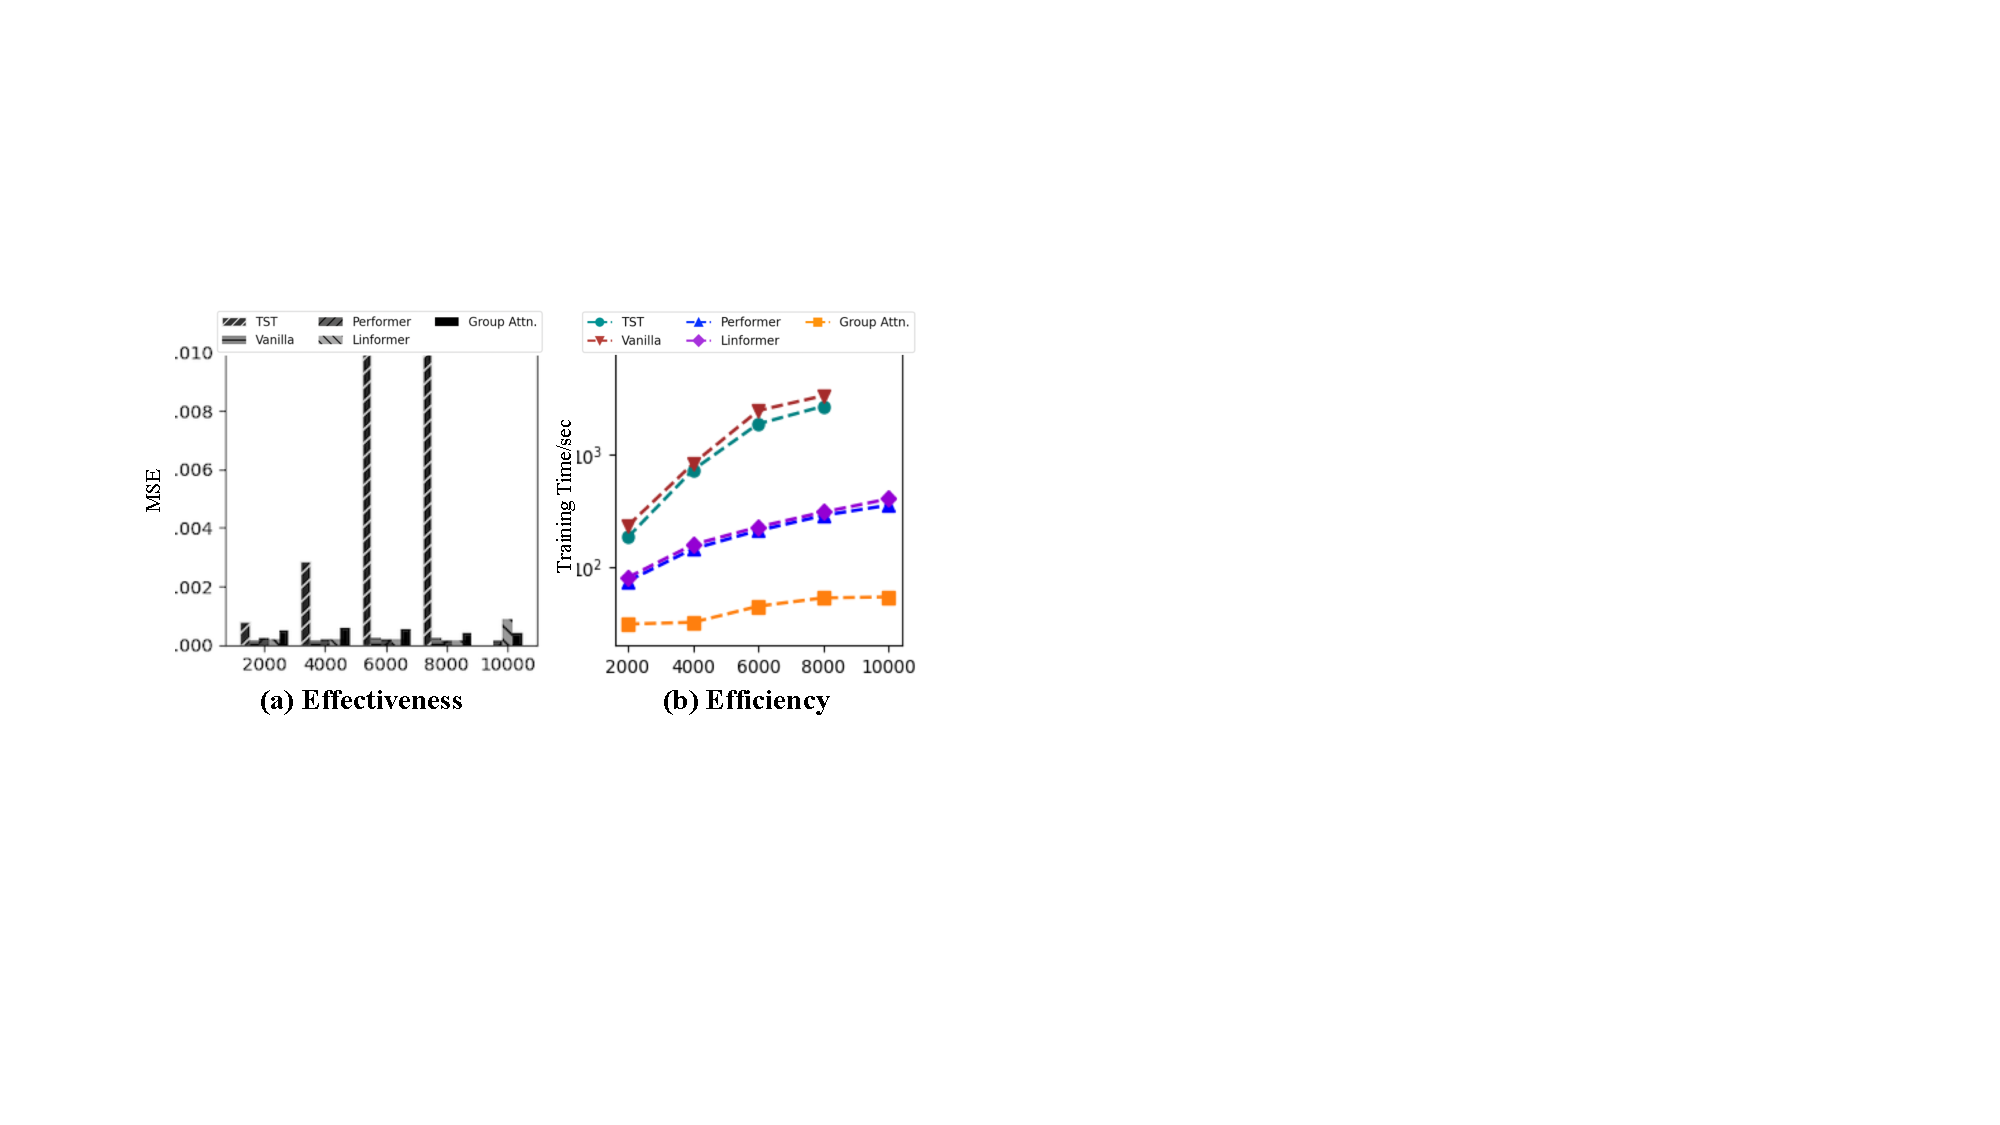
\includegraphics[width=1.0\columnwidth]{figures/line_flat.pdf}
    \vspace{-7mm}
    \caption{Varying the lengths of timeseries.}
    \label{fig.length}
    \vspace{-2mm}
\end{figure}

% \begin{figure}[t]
% %\vspace{-3mm}
%     \centering
%     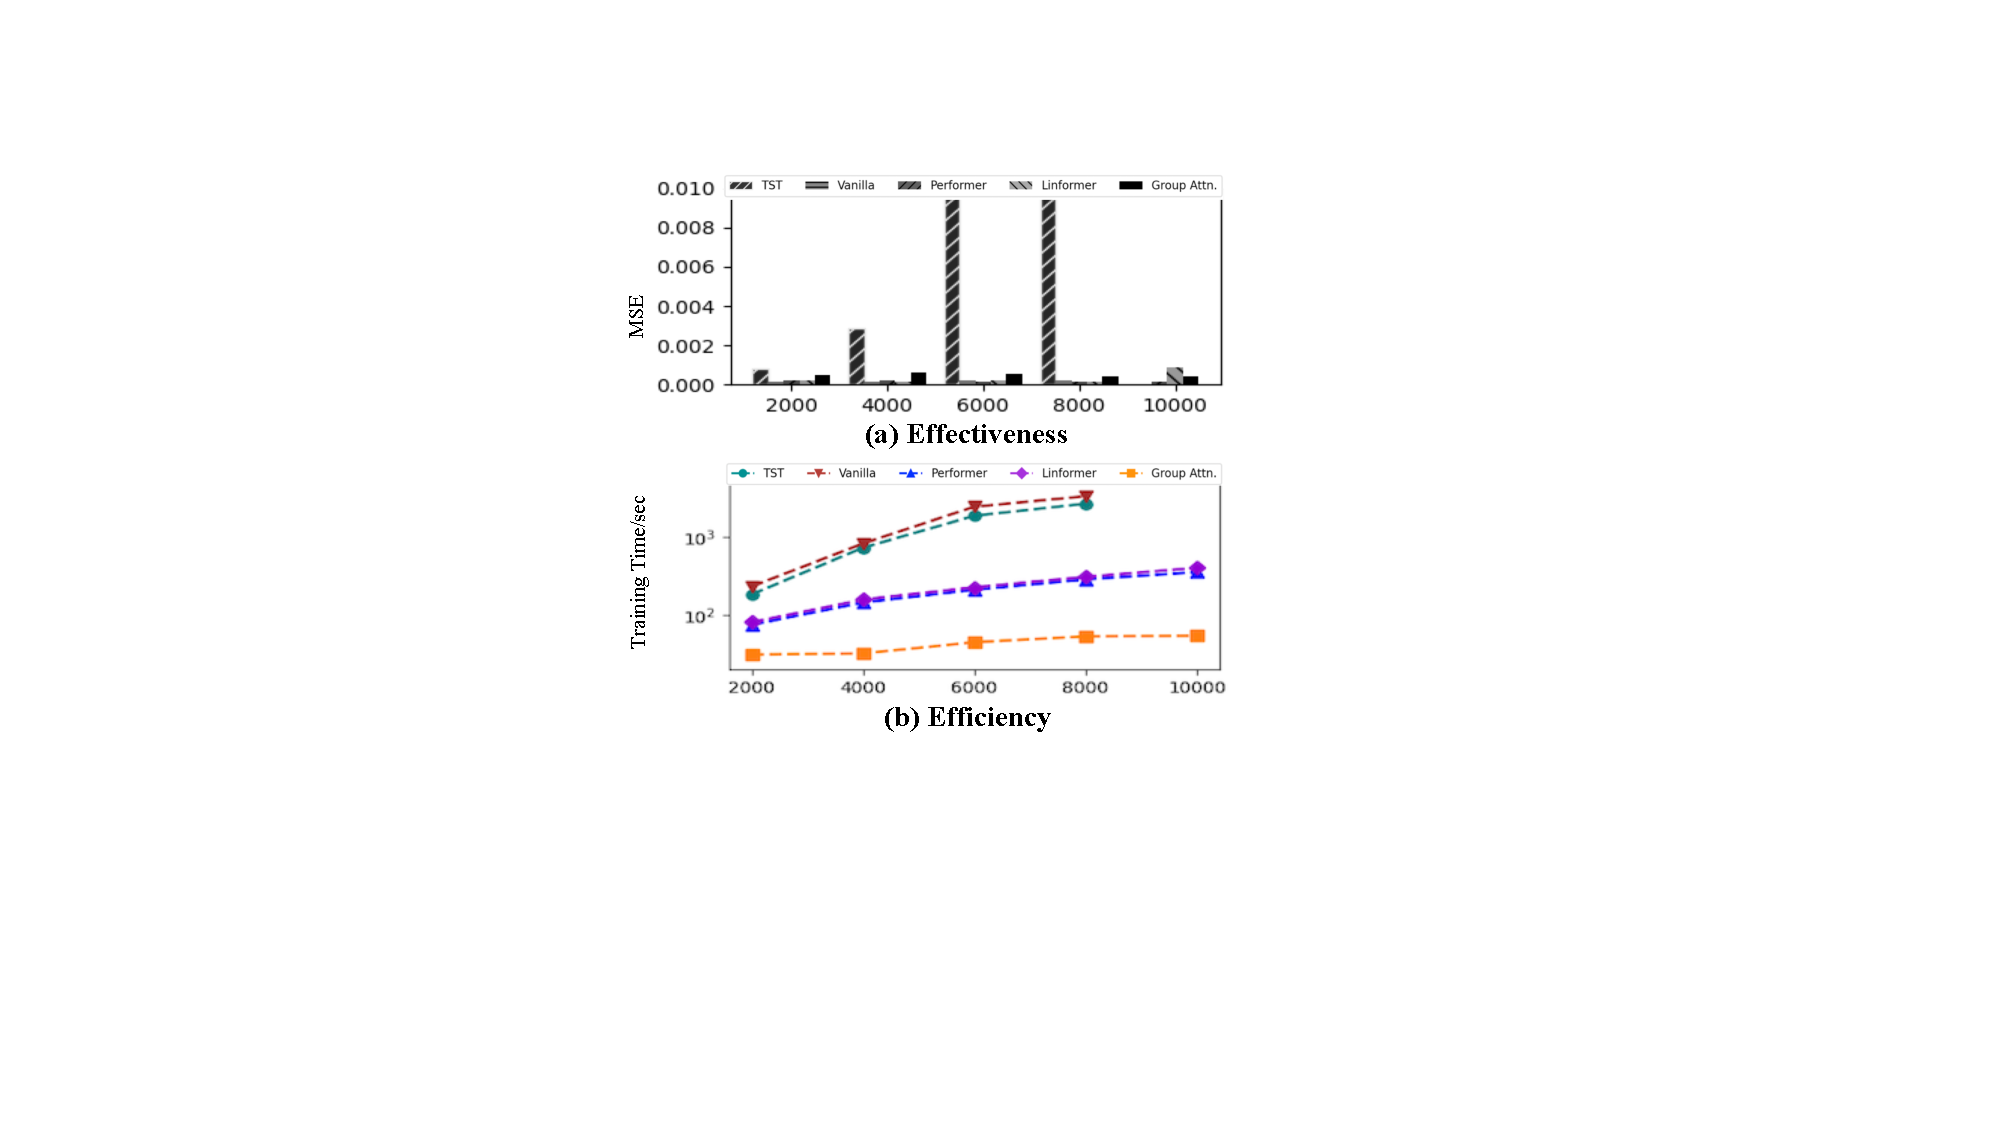
\includegraphics[width=0.8\columnwidth]{figures/line_stack.pdf}
%     \vspace{-3mm}
%     \caption{Varying the lengths of timeseries. \jm{revised: R2O3 stack}}
%     \label{fig.length}
%     \vspace{-3mm}
% \end{figure}

\subsubsection{Training time: Varying the Length\nopunct}\ \\
\label{sec.exp.efficiency.length}
In this experiment, we truncate the original MGH timseries into sequences with the lengths at 2000/4000/6000/8000/10000, and compare Group Attn. against Vanilla and other attention mechanisms. Vanilla cannot handle sequences longer than 8000.

The results in Fig.~\ref{fig.length} again show that \textit{the longer the timeseries, the larger the speed up}. With comparable MSE, Group Attn. outperforms Vanilla by 63X.
Moreover, as the length increases from 2000 to 10000, the training time of Group Attn. only increases from 31.2 seconds to 54.4 seconds per epoch.
The reason is that as the timeseires becomes longer, there are more grouping opportunities because of the similarity of the timeseries segments. 
%TST performs the worst in term of imputation error, especially when timeseries are longer. Other methods have comparably low imputation errors. 

\subsection{Comparison to Non-deep Learning Methods}
\label{sec.exp.univariate}

\begin{figure}[t]
\vspace{-2mm}
    \centering
    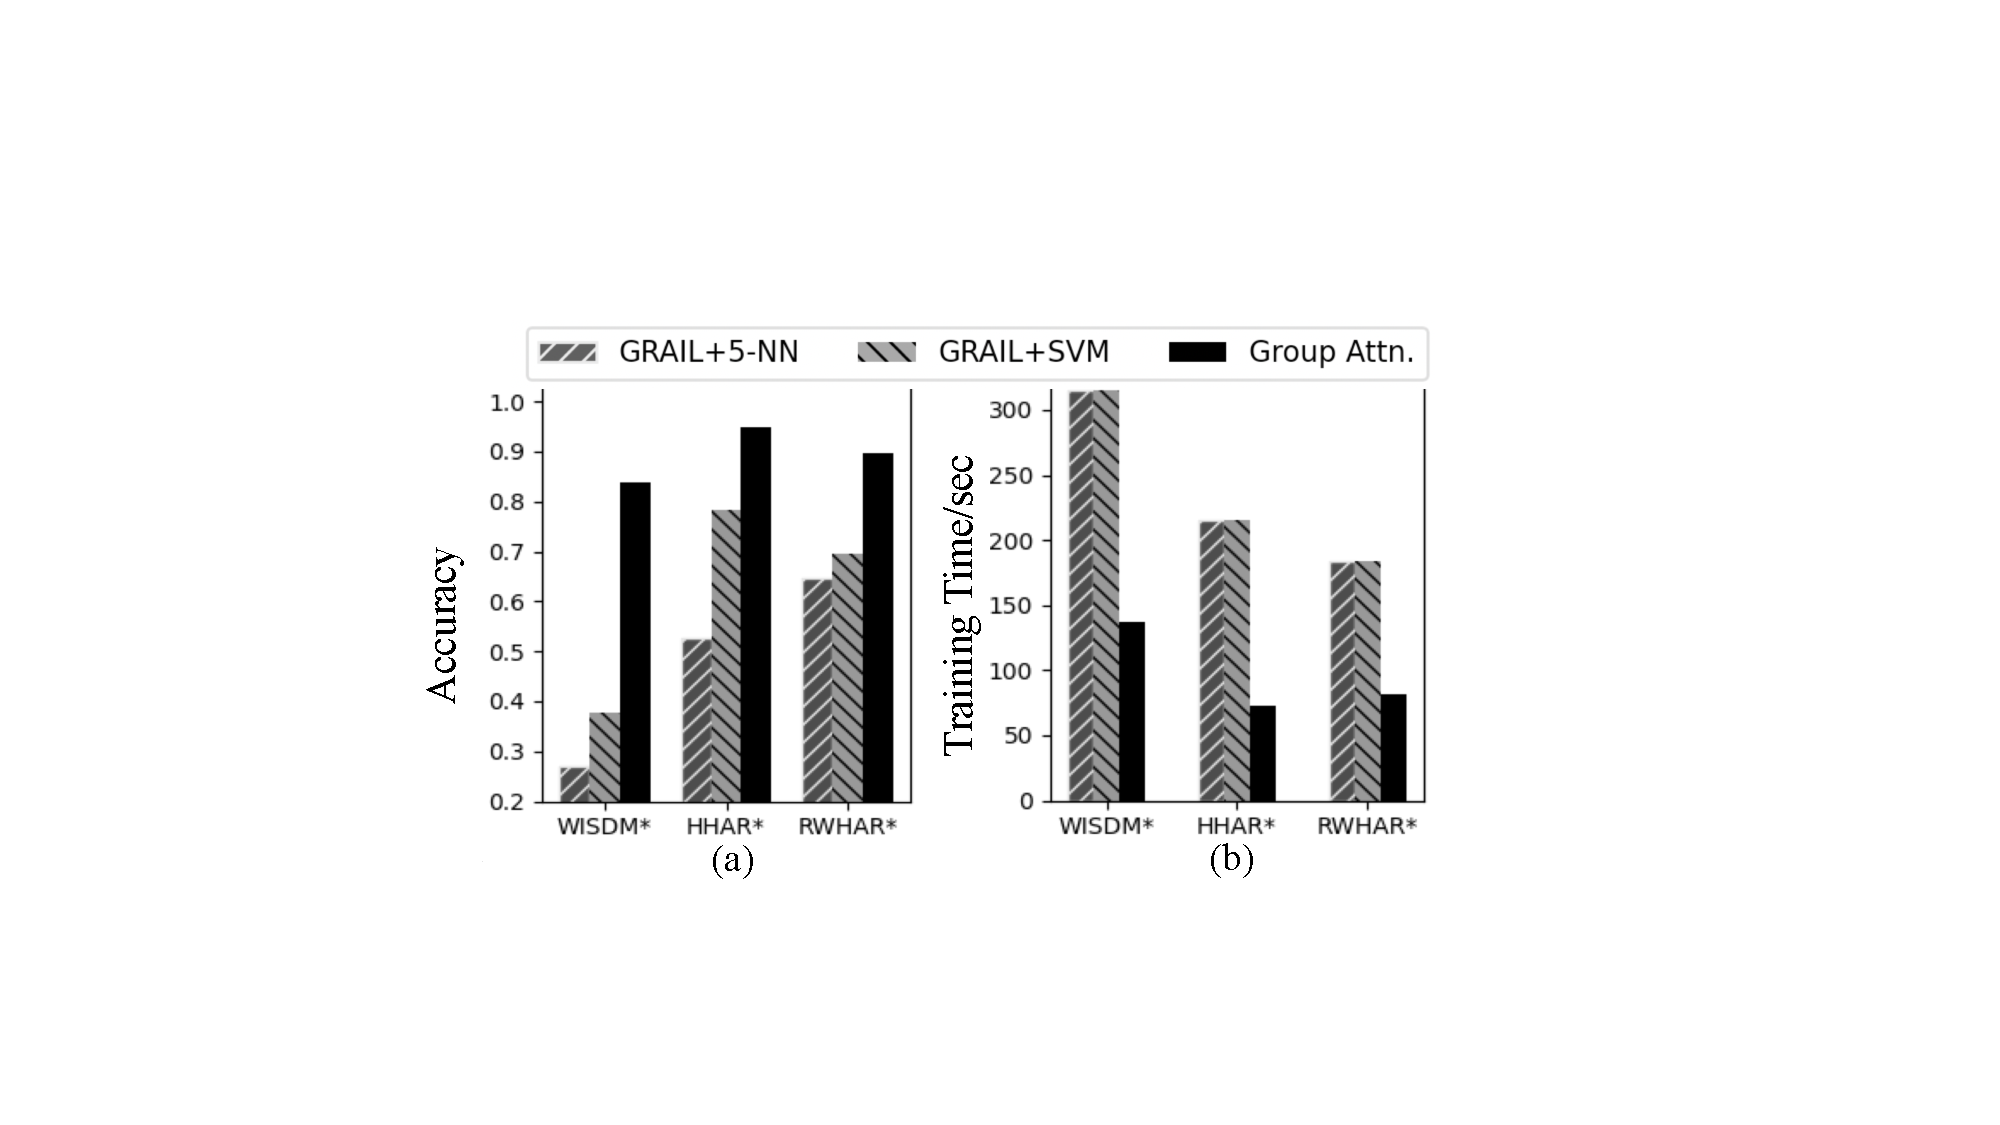
\includegraphics[width=0.8\columnwidth]{figures/uni_bar.pdf}
    \vspace{-4mm}
%    \setcaptionwidth{3.5in}
    \caption{Comparison to non-deep learning method (uni-variate data).}
    %Metric is given in accuracy on classification. Efficiency is measured by the average training time per epoch. \jm{revised}}
    \label{fig.full_uni}
    \vspace{-5mm}
\end{figure}

We compare against GRAIL, the SOTA of non-deep learning timeseries representation learning. We use the three uni-variate datasets, because GRAIL only targets uni-variate timeseries.

Results in Fig.~\ref{fig.full_uni} show that on all 3 datasets \system significantly outperforms GRAIL in accuracy by 45, 16, and 21 percentage points because of the expressive power of Transformer.
Moreover, thanks to the GPU-friendly design of \system, it is at least 2$\times$ faster than GRAIL in training time.

\subsection{Ablation Study}
\label{sec.exp.ablation}

\subsubsection{Adaptive Scheduler\nopunct}\ \\
To evaluate the effectiveness of \system's adaptive scheduler (Sec.~\ref{sec.scheduler}), we compare it against a baseline using a fixed group number $N$. We vary $N$ and the error bound threshold $\epsilon$ used by \system.   

From the results in Table~\ref{tab.dynamic} we get the following observations: 

\textbf{(1) Adaptive Scheduler is better than fixed $N$.} Training with Adaptive Scheduler already achieves better or comparable performance compared to the best performing $N$. More specifically, on the MGH dataset, dynamic scheduler always achieves better accuracy and is much faster compared to fixed $N$.
On the ECG dataset, although fixed $N$ is slightly better than adaptive scheduler in accuracy when setting the N as 512, it runs much slower than adaptive scheduler. 
Of course, finding the best $N$ that balances the accuracy and running time requires careful tuning.  
 
\textbf{(2) Adaptive Scheduler is tuning free.} It is robust on both accuracy and running time when $\epsilon$ varies, while the results of fixed $N$ vary significantly when the value of $N$ changes.
Therefore, Adaptive Scheduler frees the users from tuning the $\epsilon$ threshold, while it is hard to find an appropriate $N$ for a given dataset.


\begin{table}[htbp]
\vspace{-2mm}
\centering
\footnotesize
\begin{tabular}{cc|c|c|cc}
\toprule
Dataset & Task & Scheduler & Parameter & Metric & Time\\
 \hline
 \multirow{6}{*}{ECG} & \multirow{6}{*}{Class.} & \multirow{3}{*}{Dynamic} & 1.5 & 88.34\% & 292.5  \\
  & &  & 2 & 88.48\% & 236.8 \\
  &   &  & 3 & 87.83\% & 216.8 \\
   \cline{3-6}
   &   & \multirow{5}{*}{Fixed}  & 64 & 87.50\% & 255.2\\
   &   &   & 128 & 88.96\% & 297.2\\
   &   &  & 256 & 88.82\% & 414.1 \\
   &   &  & 512 & 90.03\% & 662.6 \\
   &   &  & 1024 & 88.65\% & 873.7\\
   \hline \hline
   
 \multirow{6}{*}{MGH} & \multirow{6}{*}{Imput.} & \multirow{3}{*}{Dynamic} & 1.5 & 0.00041 &  60.7  \\
  & &  & 2 & 0.00040  & 57.9 \\
  &   &  & 3 & 0.00042  & 54.4   \\
   \cline{3-6}
   &   & \multirow{4}{*}{Fixed}  & 128 & 0.00054 & 128.6 \\
   &   &  & 256  & 0.00053 & 190.2\\
   &   &  & 512  & 0.00049 & 240.8\\
   &   &  & 1024  & 0.00046 & 323.3 \\
 \bottomrule
\end{tabular}
%\setcaptionwidth{3.5in}
\caption{Adaptive Scheduling VS Fixed N.}
\label{tab.dynamic}
\vspace{-3mm}
\end{table}
%Parameter is error bound $\epsilon$ in Adaptive Scheduler and the number of groups $N$ in Fixed N.
%Metric is given in accuracy on classification task and mean-square error on imputation task. 



\begin{comment}


\begin{table*}[htbp]
\centering

\begin{tabular}{c|cc|cc|cc|cc|cc}
\toprule
  \multirow{2}{*}{Length} & \multicolumn{2}{c}{TST} & \multicolumn{2}{c}{Vanilla} & \multicolumn{2}{c}{Performer} & \multicolumn{2}{c}{Linformer} & \multicolumn{2}{c}{Group Attn.}  \\
  \cline{2-11}
   & MSE & Time & MSE & Time & MSE & Time & MSE & Time & MSE & Time\\
   \hline
   2000 & 0.00076 & 184.4 & 0.00014 & 232.9 & 0.00024 & 75.2 & 0.00018  & 81.0  &   0.00052 & 31.2\\
   4000 & 0.00285 & 732.1 & 0.00017 & 830.4 & 0.00019 & 145.2 & 0.00067 & 158.4 & 0.00060 & 32.3\\
   6000 & & 1879.9 & 0.00026 & 2460.6 & 0.00017 & 211.7 & 0.00015 & 227.9 & 0.00054 & 45.0\\
   8000 & & 2695.9 & 0.00026 & 3347.0 & 0.00014 & 287.8 & 0.00014 & 309.0 & 0.00042 & 53.3\\
   10000 & N/A & N/A & N/A & N/A & 0.00014 & 356.2 & 0.00088 & 404.9 & 0.00042 & 54.4 \\
 \bottomrule
\end{tabular}
\caption{Group Attention VS Vanilla: varying the lengths of timeseries (MGH data).}
\label{tab.length}
\end{table*}

\end{comment}

\begin{table}[htbp]
\vspace{-4mm}
\centering
\footnotesize
\begin{tabular}{c|c}
\toprule
 Pretrain Data size & Few-label Accuracy \\
 \hline
   N/A & 62.56\%   \\
   \hline
   12,446 & 72.94\%\\
   24,892 &  72.78\%\\
   37,338 & 74.10\%\\
   49,784 & 74.22\%\\
   62,231 & 75.06\% \\
 \bottomrule
\end{tabular}
%\setcaptionwidth{3.5in}
\caption{\system Pretraining: increasing sizes of pretrain set.}
\label{tab.pretrainsize}
\vspace{-8mm}
\end{table}

\vspace{-1mm}
\subsubsection{The Sizes of the Pretraining Data\nopunct}\ \\
Next, we evaluate how the number of unlabeled data influences the effectiveness of pretraining. 
To get empirical results, we pretrain \system on WISDM dataset with 20\%/40\%/60\%/80\% of the pretraining data and finetune each pretrained model with 100 labels per class. 
The results in Table~\ref{tab.pretrainsize} show that: 
\textbf{(1) The more pretraining data, the larger the improvement.} The accuracy increases with the sizes of the pretraining data; \textbf{(2) Marginal utility diminishing.} The first 20\% pretraining data gives a 10.38\% improvement in accuracy (72.94\% vs 62.56\%), while the remaining 80\% pretraining data only gives an additional improvement of 2.12\% (75.06\% vs 72.94\%). 

%We notice that when using all the pretraining data, there is still a gap between with full-label training (75.06\% vs. 87.05\%). However, the size of WISDM limits the possibility to further explore the ceiling benefit of pretraining (is it possible to approach full-label training accuracy?). The problem is left to be studied in future work.

\begin{comment}
\noindent\textbf{Convolutional kernal size}
\ref{tab.cnnsize}

\begin{table}[htbp]
\centering
\caption{Convolution kernal size}
\begin{tabular}{ccc|c}
\toprule
Dataset & Task & Kernel Size  & Metric\\
 \hline
 ECG & Class. & & \\
 \hline \hline
 MIT-MGH & Imupt. & & \\
 \bottomrule
\end{tabular}
\label{tab.cnnsize}
\end{table}
\end{comment}

\begin{comment}

\noindent\textbf{LSH VS K-means.}
We conduct this experiments to show why K-means is a good option to group the window in Group Attn. 
We compare K-means against Locality Sensitive Hashing (LSH), because LSH does not use the number of groups as an explicit hyper-parameter. However, we have set for LSH the hyper-parameter W which controls the locality sensitivity of the hash function. We also report the results on Vainlla as the reference point.

The results are showed in \ref{tab.lshkmeans}. $N$ denotes the number of groups that each method produces.
Because vanilla Self-Attention does not group the similar windows, its $N$ is equal to the length of the sequence which is 200 in this case. 
In K-means, as a hyper-parameter, $N$ represents the number of groups we expect to produce. In LSH, $N$ corresponds to the number of groups the hash functions produce. Because different attention heads could produce different number of groups, we report the average number of groups as the $N$.  
We also report the key hyper-parameter used by each method, corresponding to the `Parameter' column in the table. In K-means, it is the maximal rounds of iterations. In LSH it is the hyper-parameter $W$. 

The results show that: \textbf{(1) K-means is very effective}. Setting $N$ as 64, Group Attn. is able to get an accuracy comparable to vanilla Self Attention after one round of learning. 
When setting $N$ to 16 (less than 1/10 of the sequence length) the accuracy only drops by 1.98\%. 
These results confirm the robustness of K-means in Group Attention;
\textbf{(2) LSH has to produce a lot of groups to get accurate result.} 
Only after we set $W$ to an extremely small value 0.01 which indicates a very strong requirement on the data locality per group, LSH gets an accuracy close to K-means with 16 groups. However, in this case it produces 172 groups in average, while the length of the timeseries is only 200. 
This leads to long training time, as the time complexity of Group Attn. is proportional to the number of groups. 

\begin{table}[htbp]
	\centering
	
	\begin{tabular}{ccc|c}
		\toprule  
		Method & N & Parameter & Accuracy \\
		\hline
		vanilla & 200 & - & 87.71\% \\
		\hline
		Kmeans & 16 & 1 & 85.37\% \\
		Kmeans & 64 & 1 & 87.53\% \\
		\hline
		LSH & 83 & 0.1 & 78.40\% \\
		LSH & 116 & 0.05 & 82.39\% \\
		LSH & 172 & 0.01 & 86.21\% \\
		\bottomrule 	
		\end{tabular}
	\caption{LSH vs. Kmeans on WISDM.}
	\label{tab.lshkmeans}
\end{table}
\end{comment}




















